% !TeX spellcheck = en_US
\documentclass[]{scrartcl}

\usepackage{graphicx}
\usepackage{amsmath}
\usepackage{hyperref}
\usepackage{comment}
%opening
\title{Lab 3}
\author{}

\begin{document}

\maketitle

\begin{abstract}

\end{abstract}

\section{R2. Anomaly detection}\label{sec:R2}
\subsection{R2.a) Anomaly detection function}\label{sec:r2a}
The function \texttt{anomalyR2a.m} was developed to detect anomalies in a time series. An anomaly is flagged if the absolute value of the difference between the predicted and given time series is greater than a threshold value. Analyzing the error in the training data, depicted in Fig. [Ref Fig. de $e(n)$], which does not seem to contain anomalies, the threshold value was chosen to be $t_a = 0.1$.


\subsection{R2.b) Test data prediction and anomaly detection}\label{sec:r2b}
The test data was uploaded and the long-term and residue prediction were computed, making use of the model found in Section [Ref Fig. de R1.]. Fig. \ref{fig:R2b_test} depicts the comparison of the test data and the long term prediction. Fig. \ref{fig:R2b_residual} depicts the comparison of the test residues and their prediction. 
\begin{figure}[htbp]
	\centering
	\begin{minipage}[b]{.49\textwidth}
		\centering
		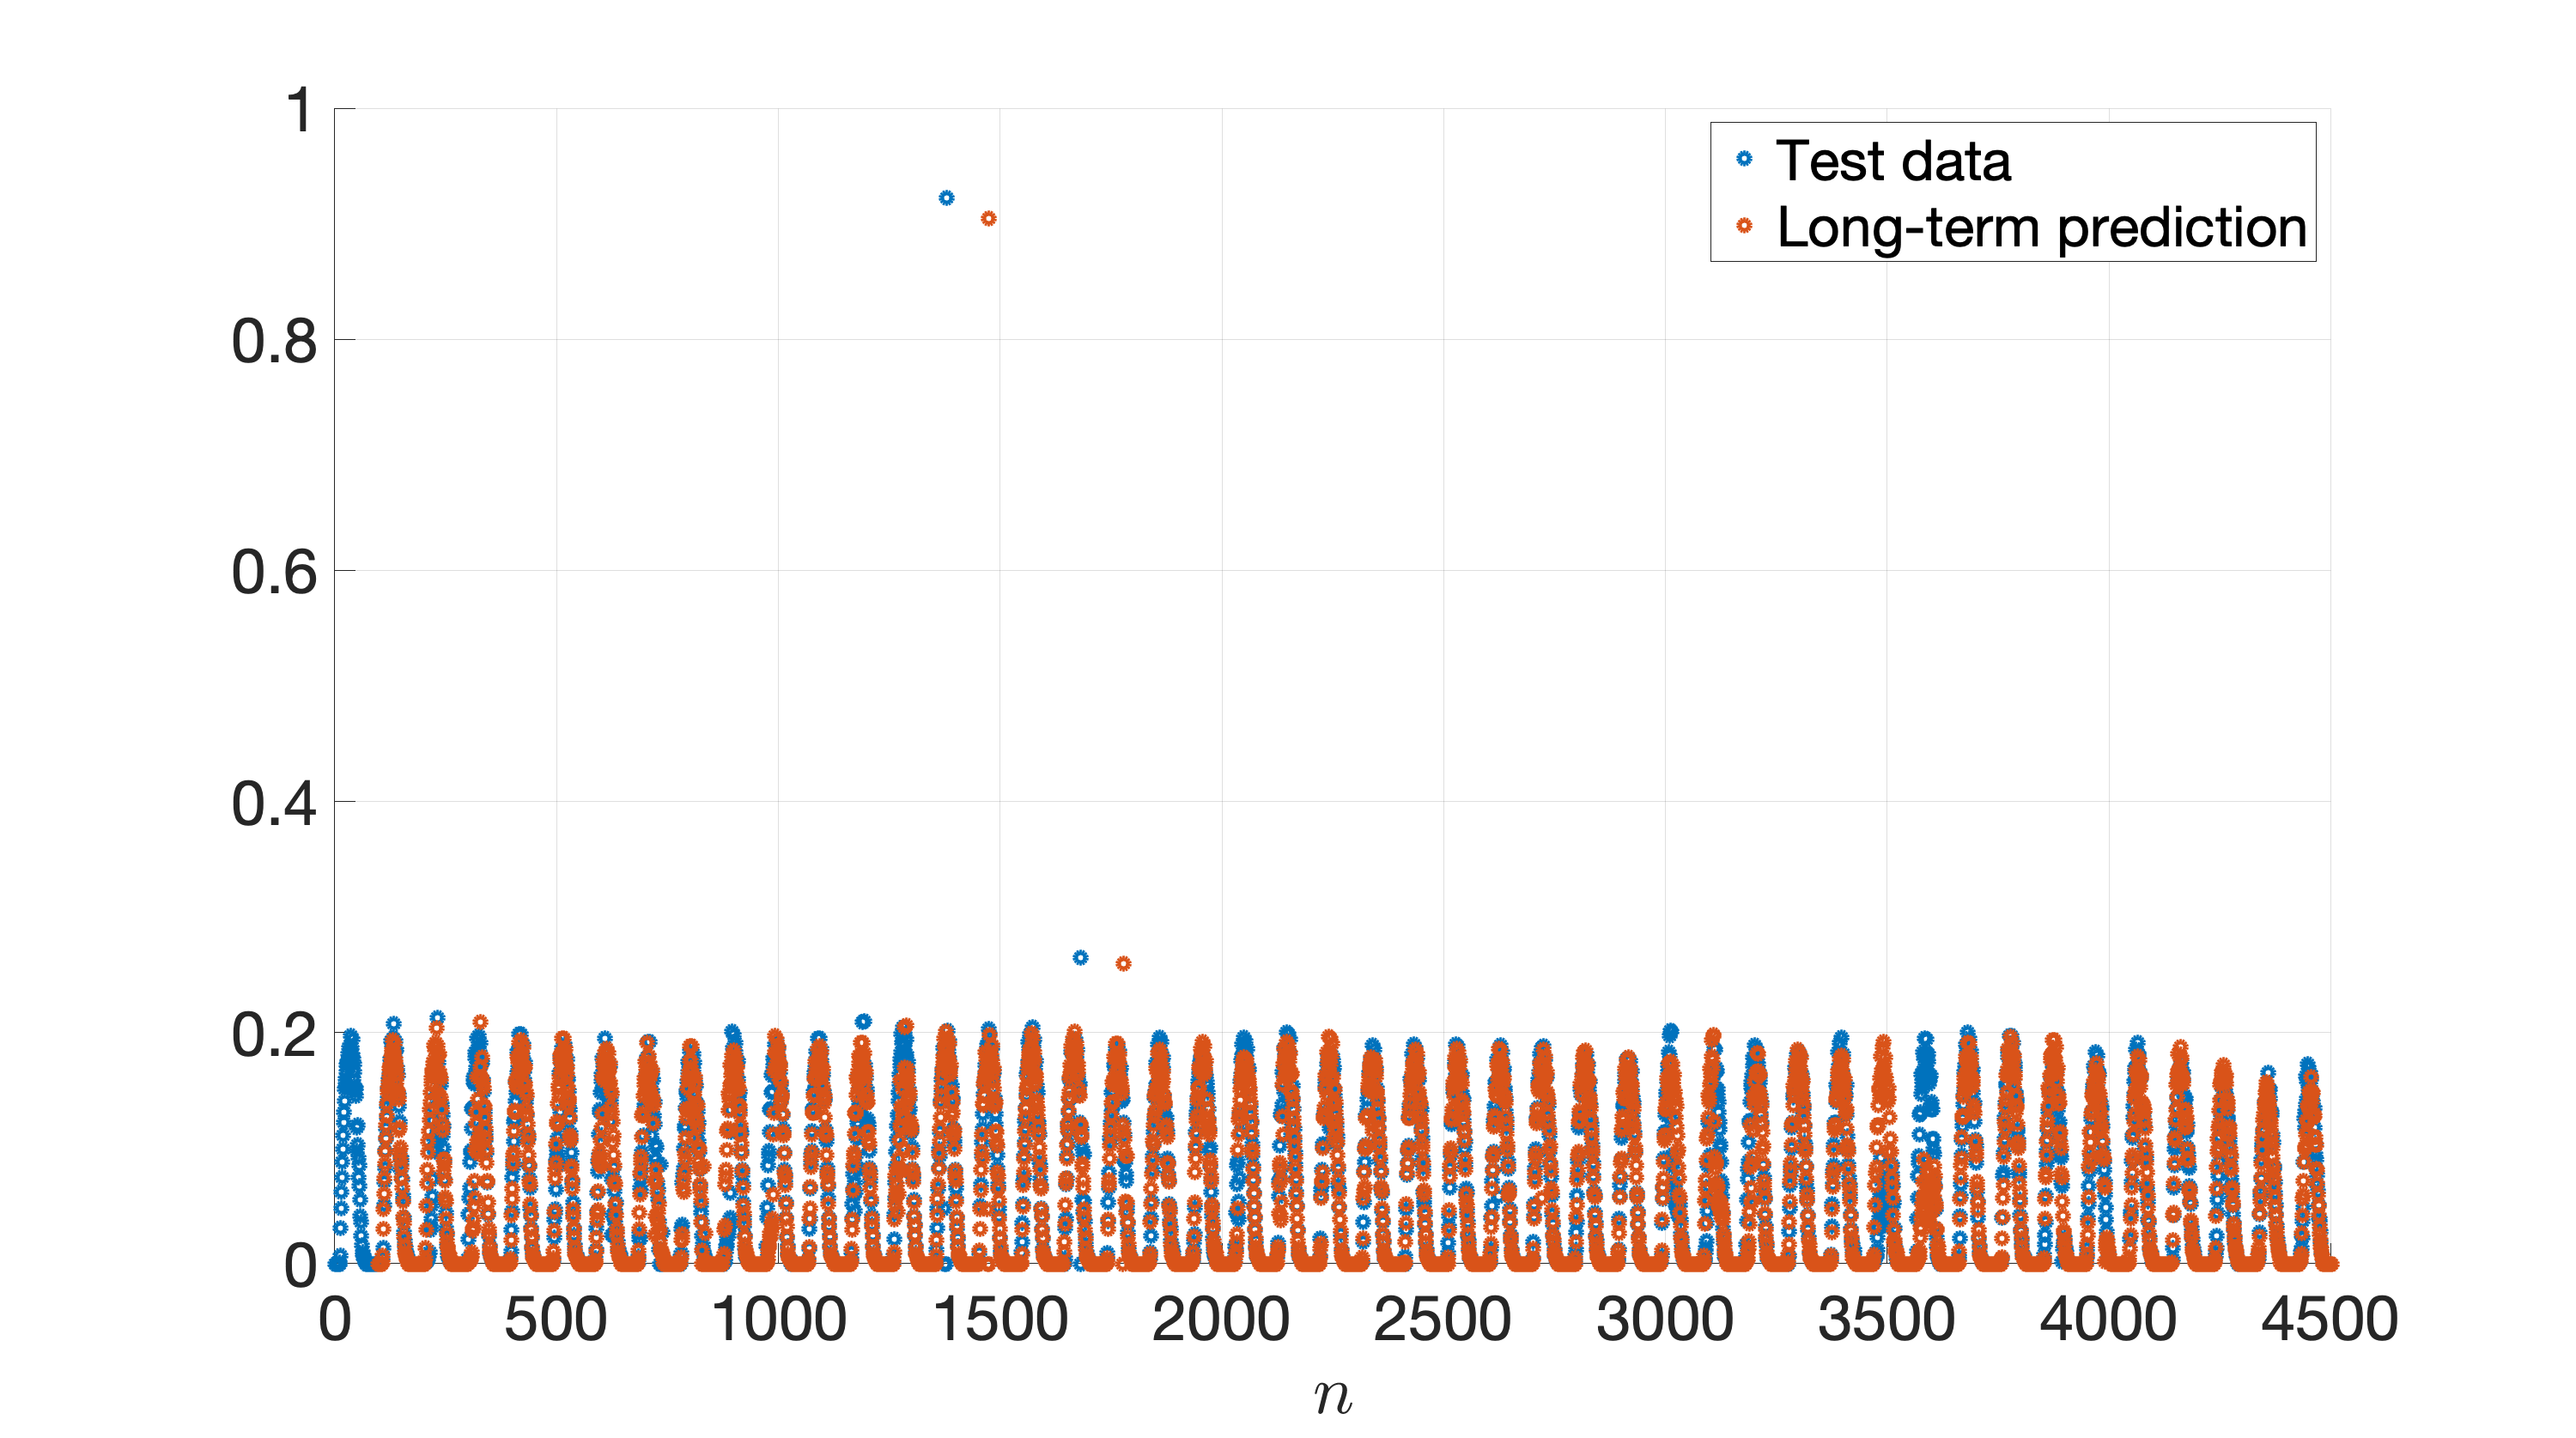
\includegraphics[width= 1.1\textwidth]{figures/R2b_test.png}
		\caption{Comparison of test data with long-term prediction.}
		\label{fig:R2b_test}
	\end{minipage}
	\hfill
	\begin{minipage}[b]{.49\textwidth}
		\centering
		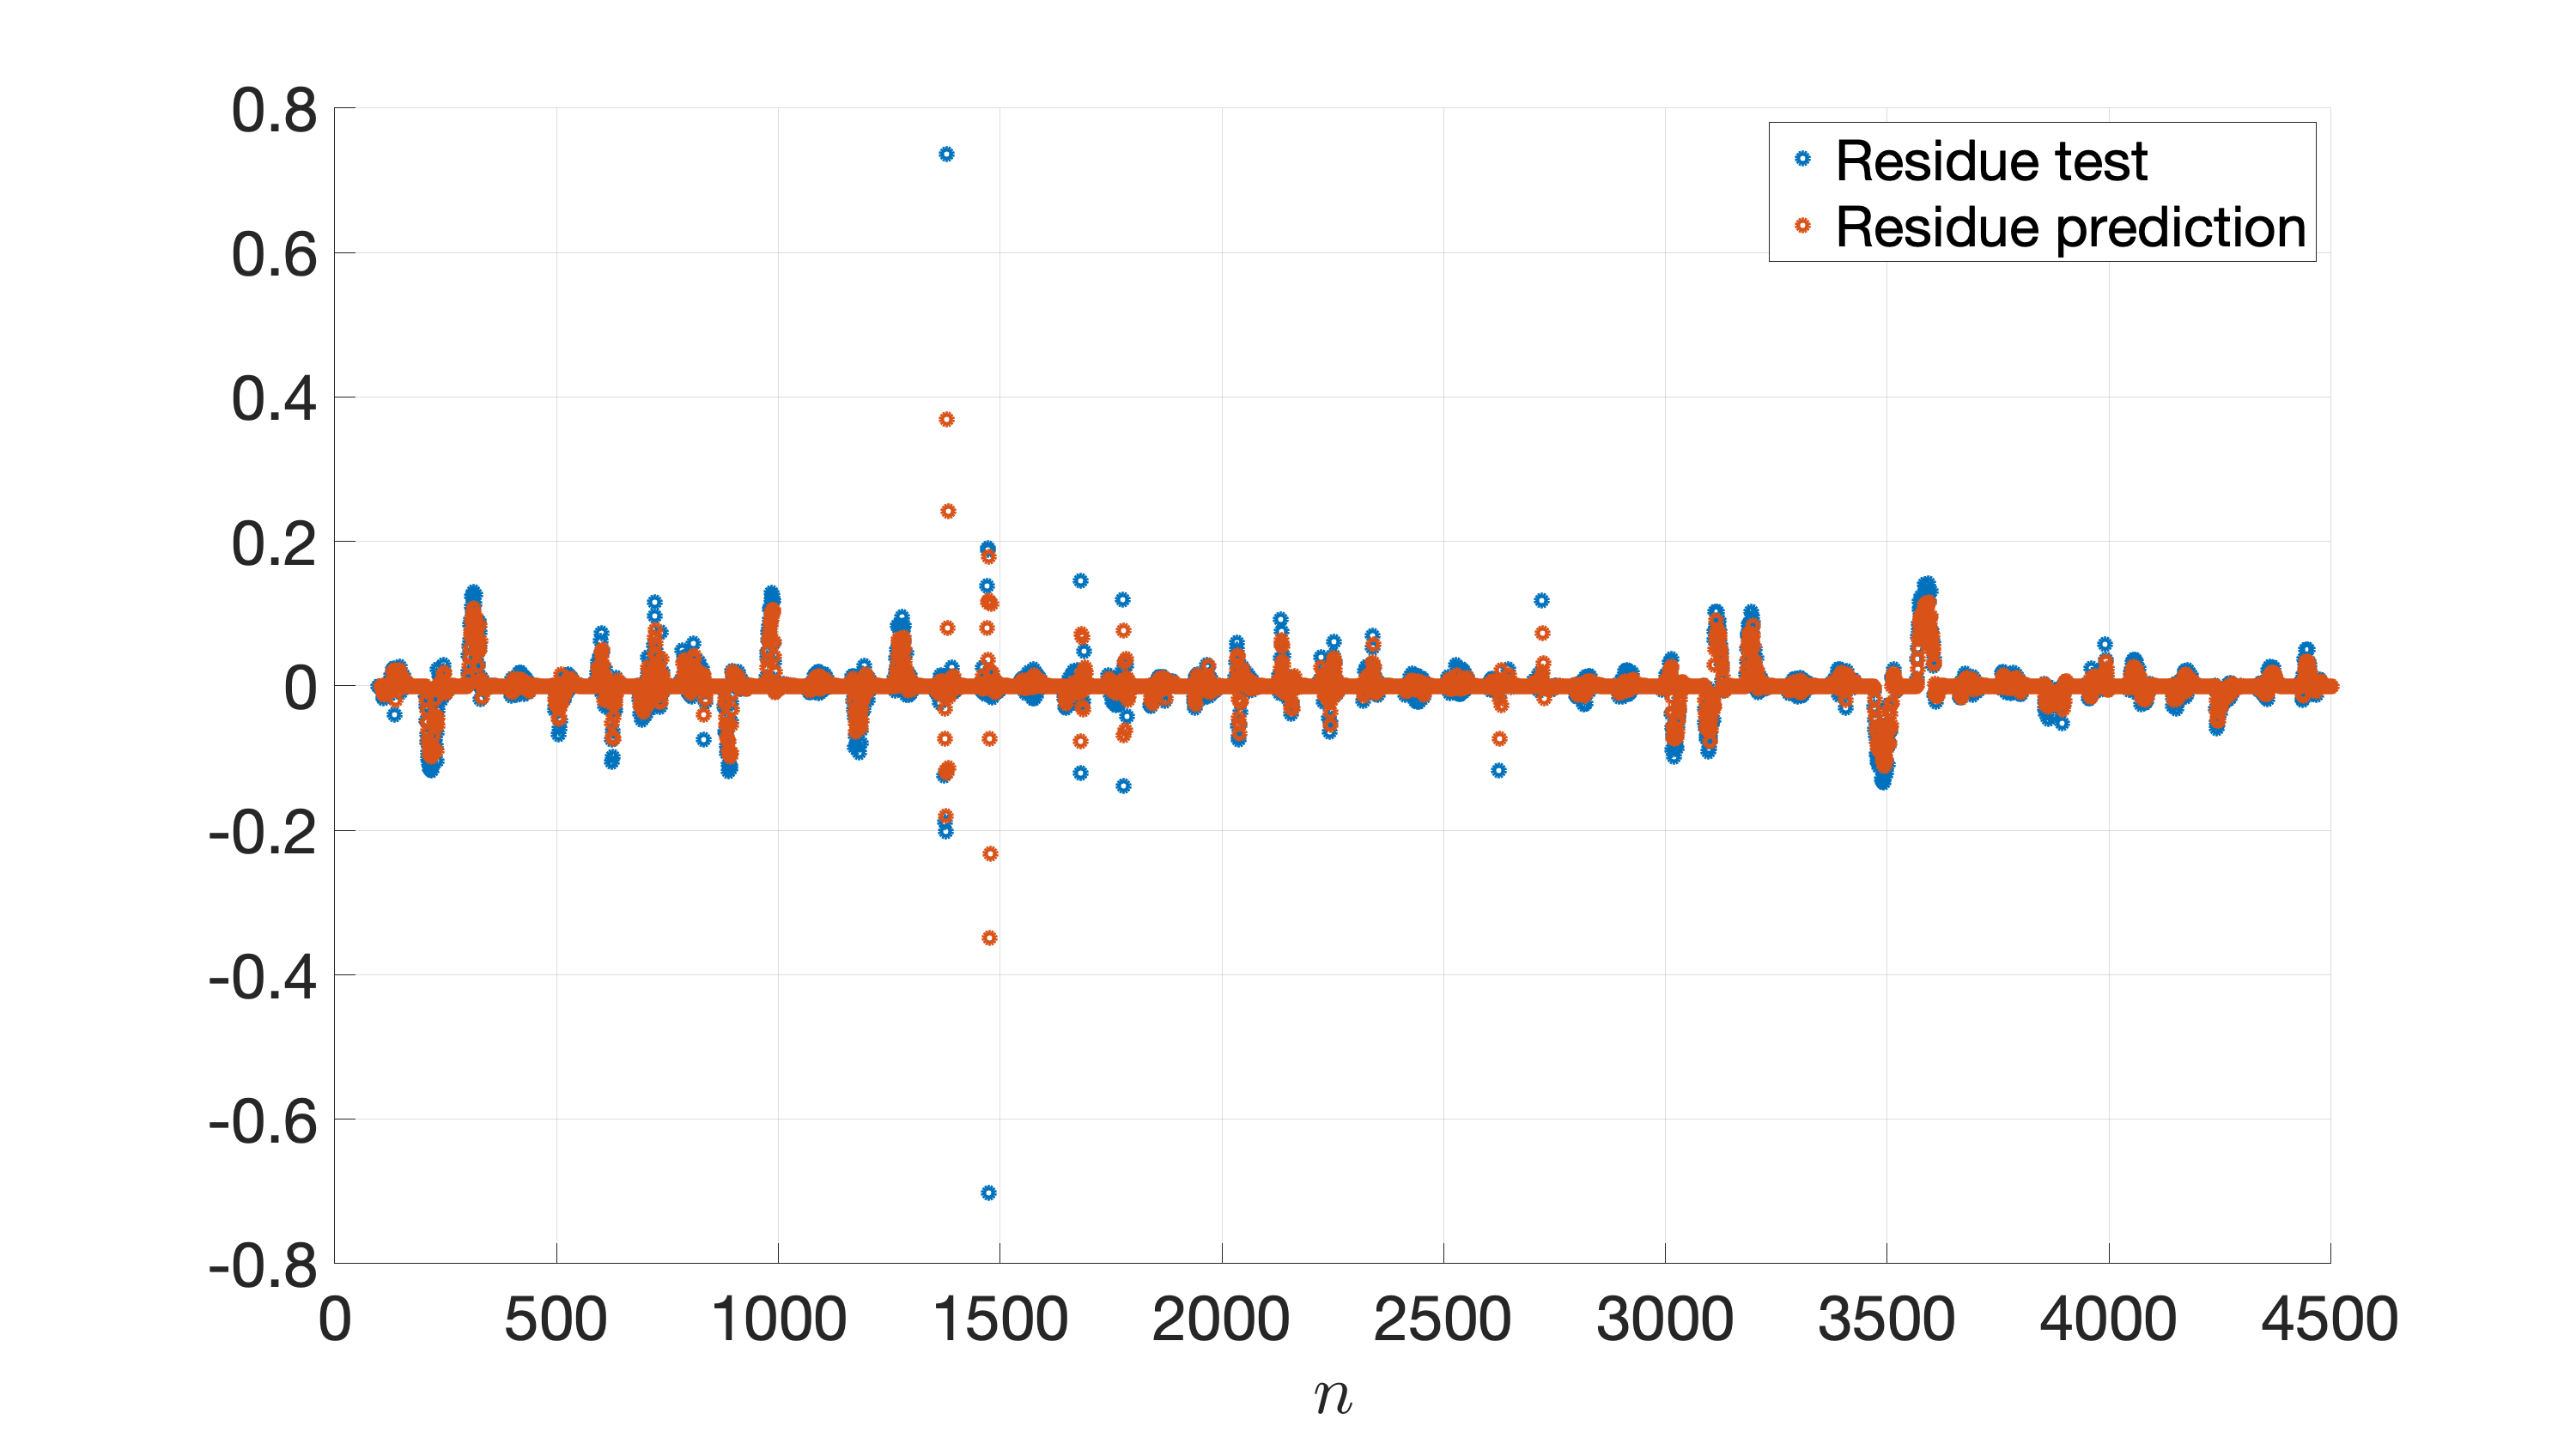
\includegraphics[width= 1.1\textwidth]{figures/R2b_residual.png}
		\caption{Comparison of test residues with their  prediction.}
		\label{fig:R2b_residual}
	\end{minipage}
\end{figure}

Evaluating the residue prediction error it is possible to apply the function developed in Section \ref{sec:r2a} to detect anomalies. Fig. \ref{fig:R2b_error_an} depicts the evolution of the residue prediction error and the anomalies identified. The dashed horizontal bars represent the anomaly threshold. 
\begin{figure}[htbp]
	\centering
	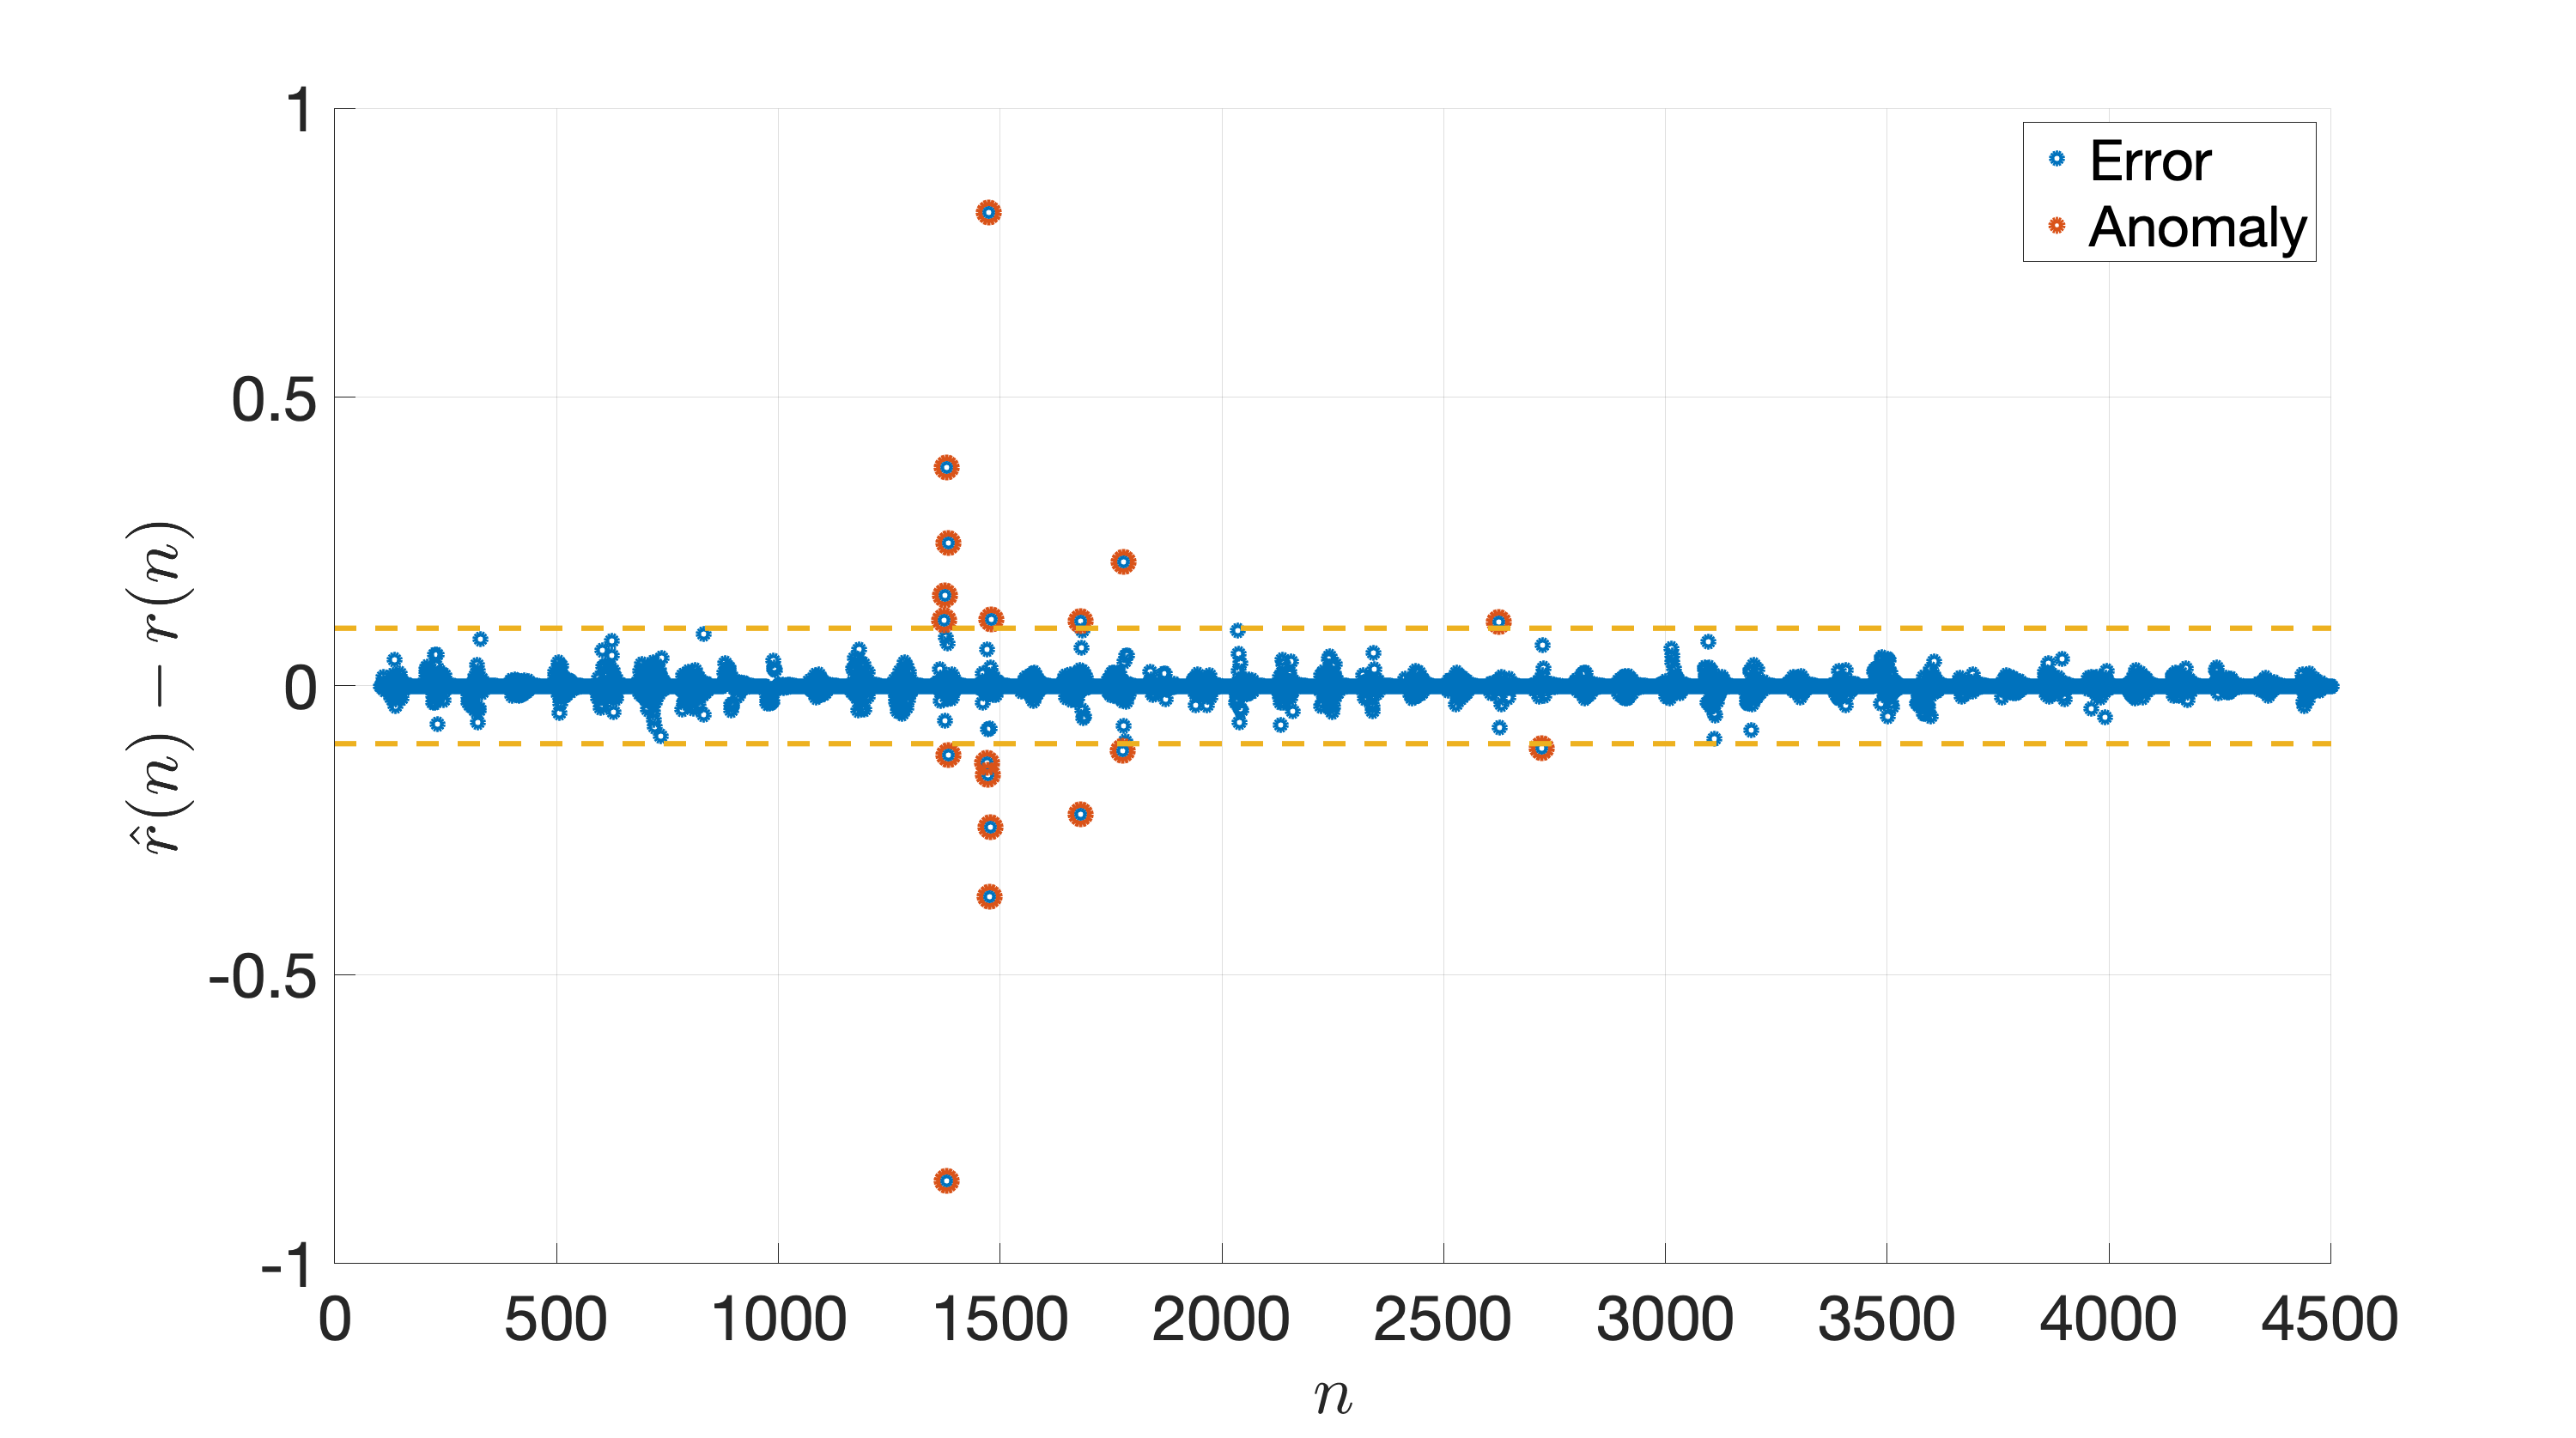
\includegraphics[width= 0.8\textwidth]{figures/R2b_error_an.png}
	\caption{Residue prediction error and anomaly identification.}
	\label{fig:R2b_error_an}
\end{figure}

First, it is interesting to analyze the ability of each of the predictions stages with regard to their ability to detect anomalies. Figs. \ref{fig:R2b_test_an} and \ref{fig:R2b_residual_an} depict the prediction of both stages as well as the test data, with the anomalies identified. On one hand, it is possible to notice that it is very difficult to point out the anomalies in the long-term model. For instance, for $n \approx 3590$, the prediction clearly deviates from the test data, and yet, it is not flagged as an anomaly. There are, however, two clear exceptions of isolated points that clearly are outliers, and, thus flagged as an anomaly. On the other hand, it is very clear in the residues prediction that there are several data points that fall out of the regular distribution of data. In this case, the outliers coincide with the flagged anomalies. The short-term model is, thus, able to flag the anomalies more clearly. Second, it noticeable that the anomalies are identified in pairs of days. Although, it is legitimate that anomalies are flagged in consecutive days, it may well be possible that the long-term prediction of the day after the first anomalies is detected is contaminated with the anomaly of the first day. If this is the case, even thought there is no actual anomaly in the day following the fist anomaly, this contamination leads to falsely flagging an anomaly. This problem is addressed in the following section, so that it is possible to understand if there are, in fact, genuine anomalies in consecutive days or if it is just the effect of the anomaly in the previous day.
\begin{figure}[htbp]
	\centering
	\begin{minipage}[b]{.49\textwidth}
		\centering
		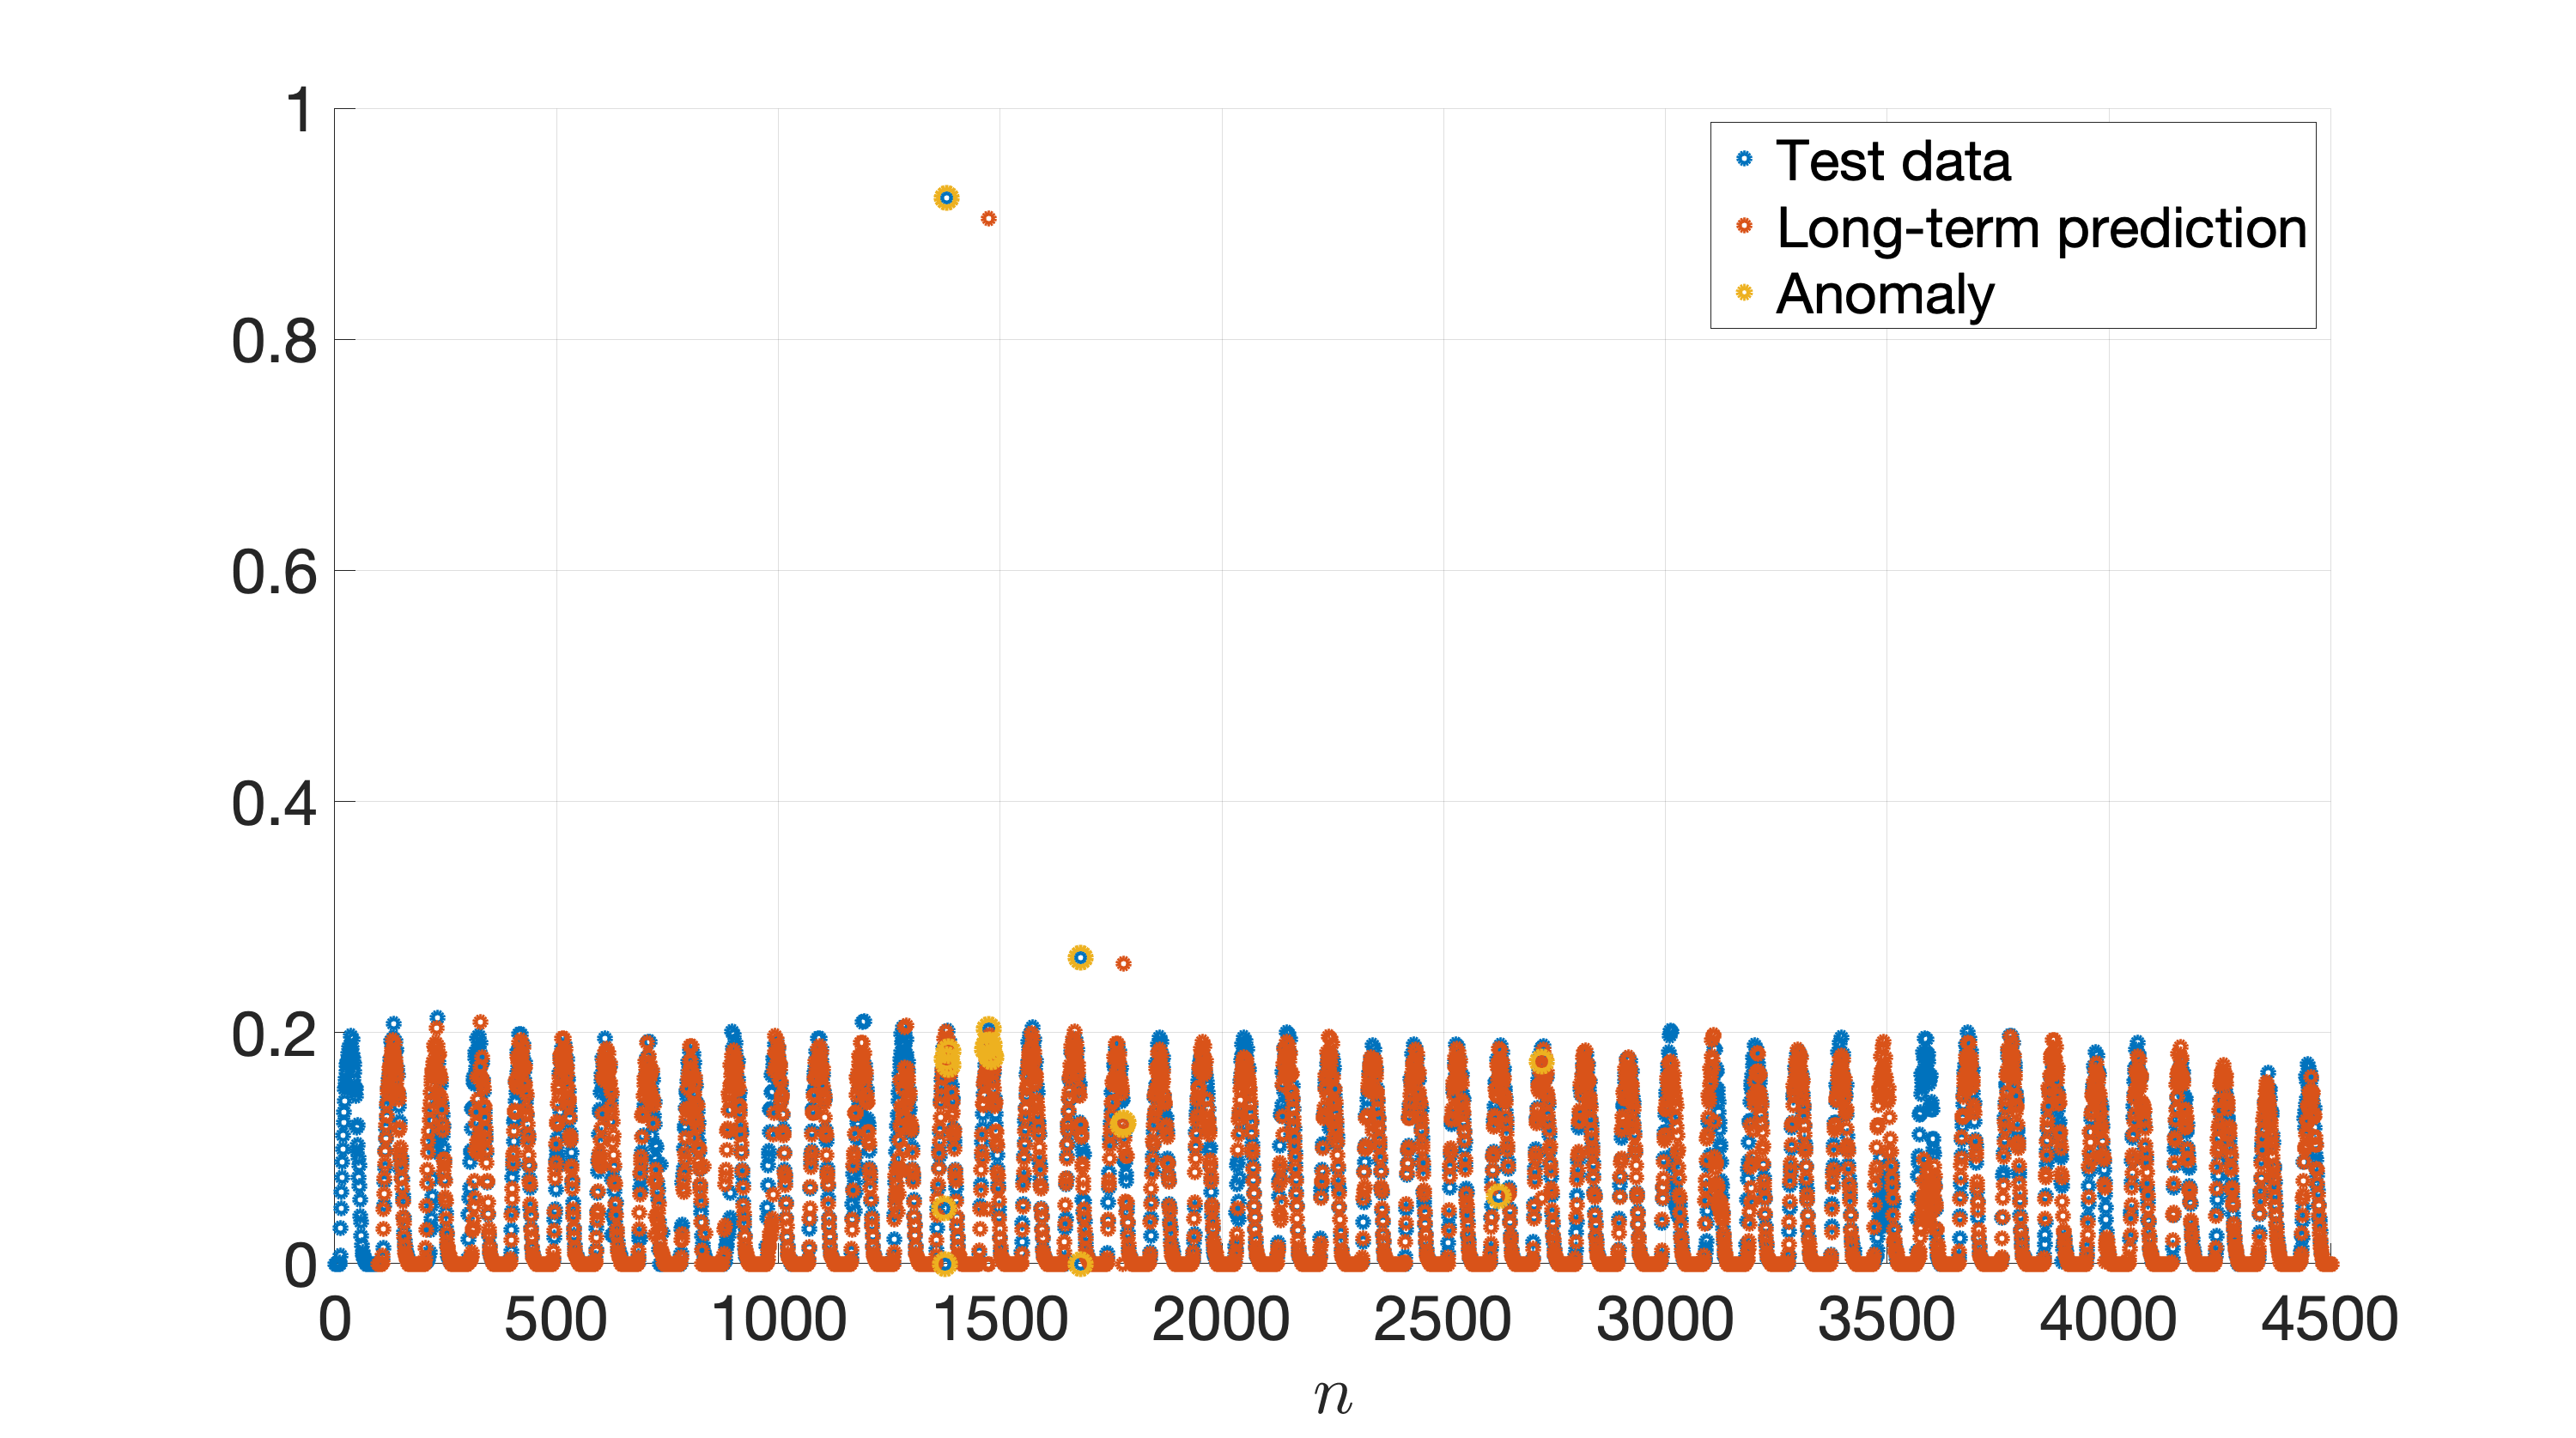
\includegraphics[width= 1.1\textwidth]{figures/R2b_test_an.png}
		\caption{Comparison of test data with long-term prediction with anomaly identification.}
		\label{fig:R2b_test_an}
	\end{minipage}
	\hfill
	\begin{minipage}[b]{.49\textwidth}
		\centering
		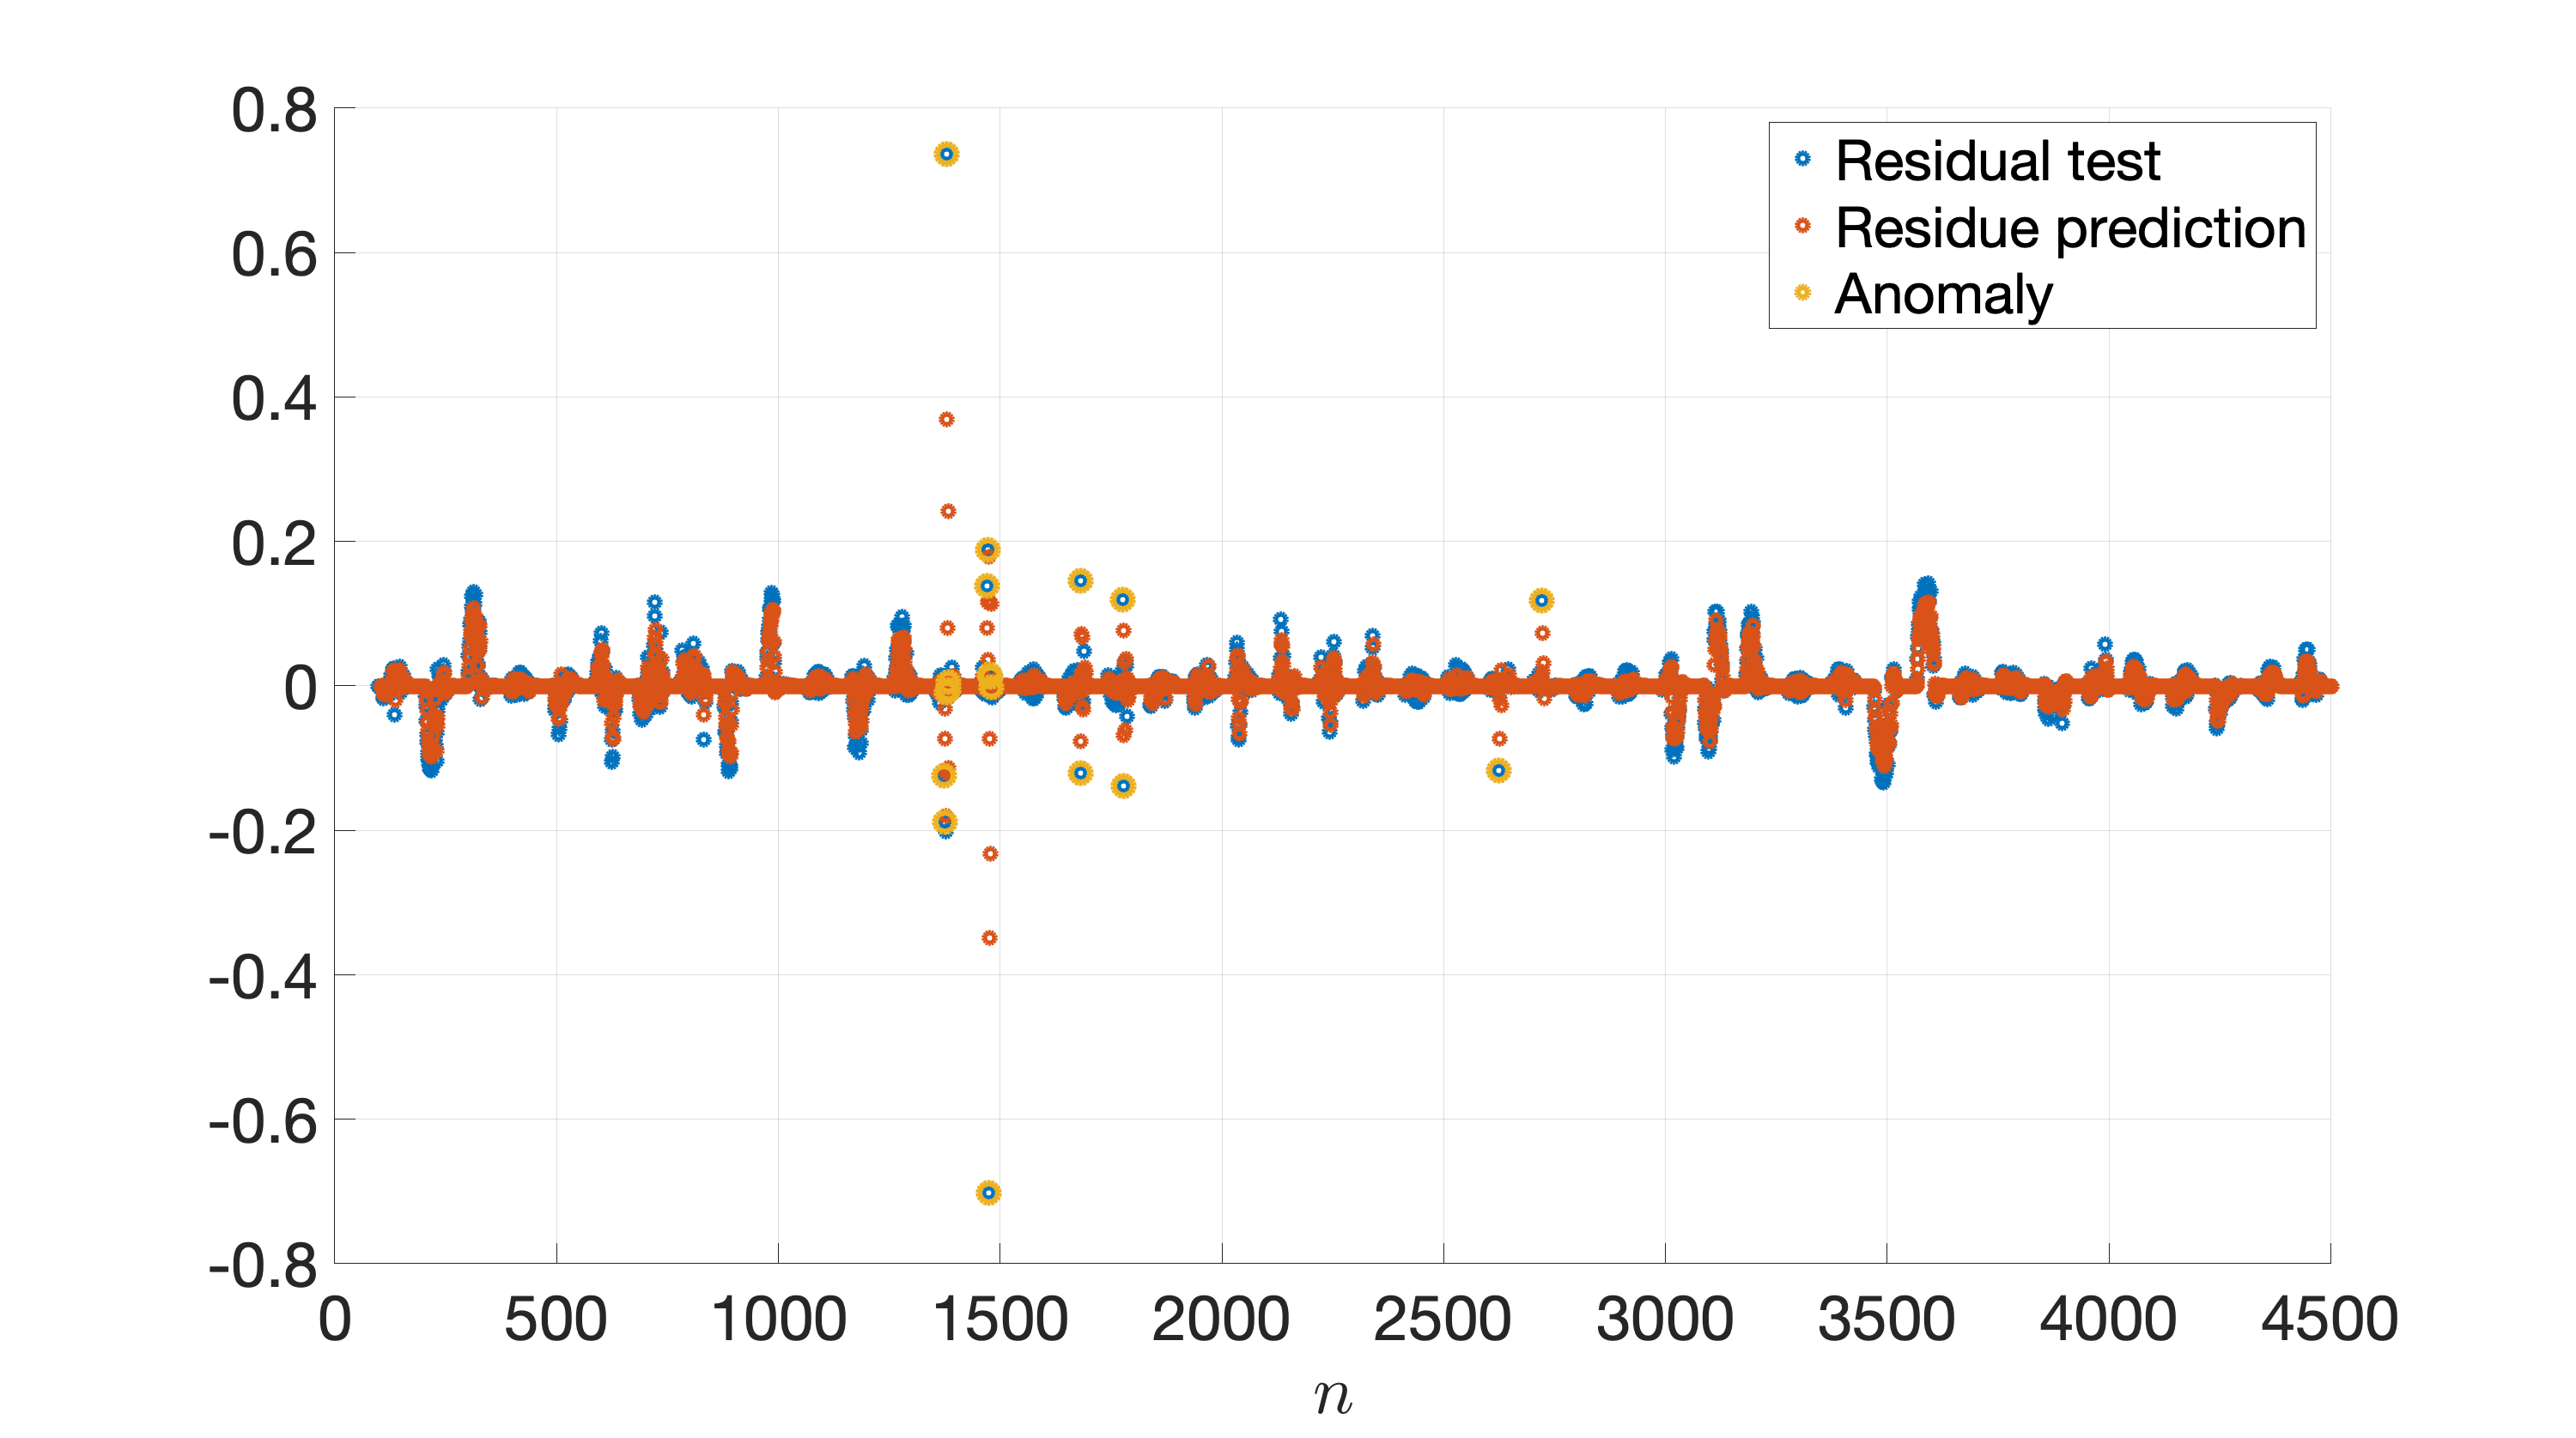
\includegraphics[width= 1.1\textwidth]{figures/R2b_residual_an.png}
		\caption{Comparison of test residues with their prediction. with anomaly identification.}
		\label{fig:R2b_residual_an}
	\end{minipage}
\end{figure}

\subsection{R2.c) Data decontamination in the event of an anomaly}
It was pointed pointed out in Section \ref{sec:r2b}, the anomalies are flagged in pair of days. For this reason, in this section it is verified if these are, in fact, genuine anomalies in consecutive days or if it is just the effect of the anomaly in the previous day. There are many ways to attenuate the dependence on the day of the first anomaly on the following days. In this laboratory report two methods are presented: i) one which is more general and suitable to be applied to more complex models than the one at hand; and ii) the outline of a method which is simpler and is devised for the particular model found in this laboratory.

The first method follows three steps. First, the intervals of time which are, without doubt, contaminated with an anomaly are identified. In this case it was considered that all the data points of a day when the first anomalies are flagged, are contaminated. Fig. \ref{fig:R2c_error_an} shows the data points of the test data which are considered to be, without doubt, contaminated by an anomaly. Again, the horizontal dashed lines in this figure represent the anomaly detection threshold. Second, an iterative procedure is followed so that the test data in the contaminated regions is substituted with data that corresponds to the prediction with the model obtained. For that reason, each iteration is made up of two steps: i) the test data, which was considered to be contaminated, is substituted by the previous prediction; and ii) the test set is predicted again with the previously updated test data set. This iteration is performed until convergence is reached. Third, the predicted data is compared with the original test data set, and the residue prediction error is evaluated with the routine designed in Section \ref{sec:r2a} to identify the anomalies. The anomalies detected in this step are now real anomalies that are not artificially caused by the anomalies identified in the first step. In the code provided these steps are commented carefully and clearly divided. The residue prediction error after these three steps can be seen in Fig. \ref{fig:R2c_error_an_after}. It is very interesting to note that, contrarily to what is seen in the anomaly identification in Fig. \ref{fig:R2b_error_an}, the second anomaly region in each of the three pairs of anomalies is no longer flagged as an anomaly. This confirms the suspicion that the second anomalies being flagged in the previous section were artificially flagged, because of the dependence on the previous day, which was anomalous. 

\begin{figure}[htbp]
	\centering
	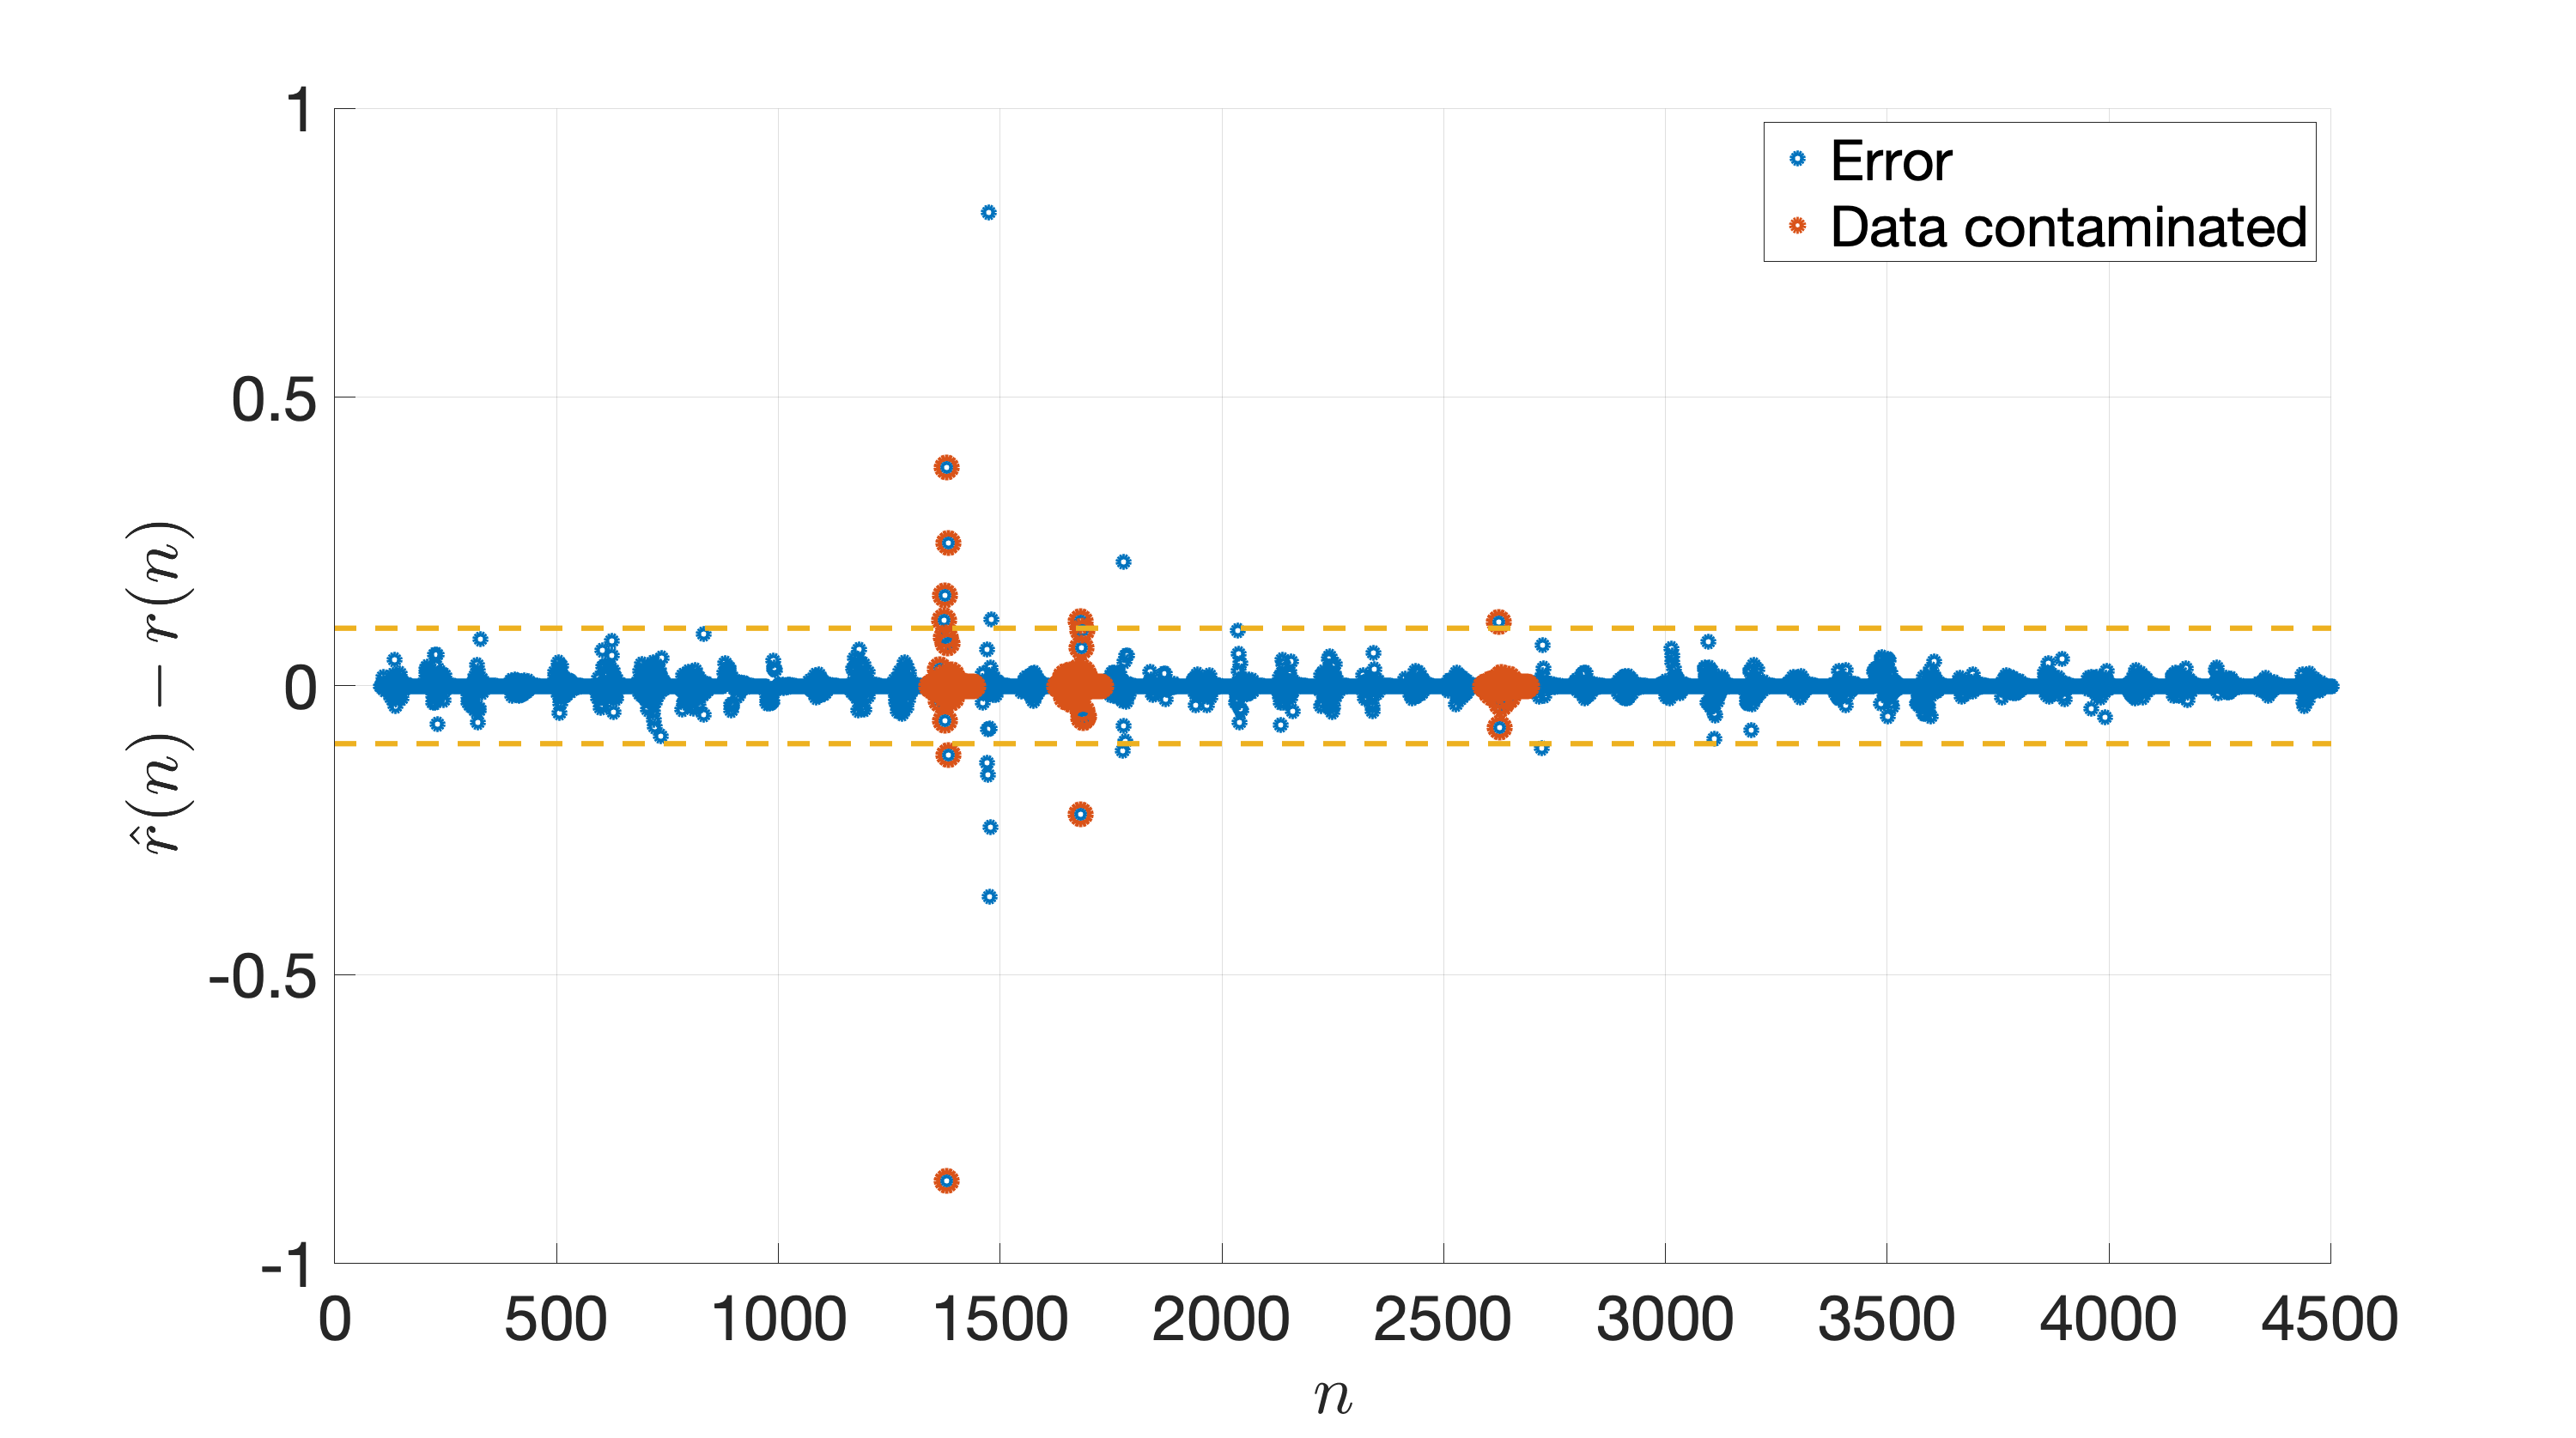
\includegraphics[width= 0.8\textwidth]{figures/R2c_error_an.png}
	\caption{Residue prediction error and first anomaly region identification.}
	\label{fig:R2c_error_an}
\end{figure}

\begin{figure}[htbp]
	\centering
	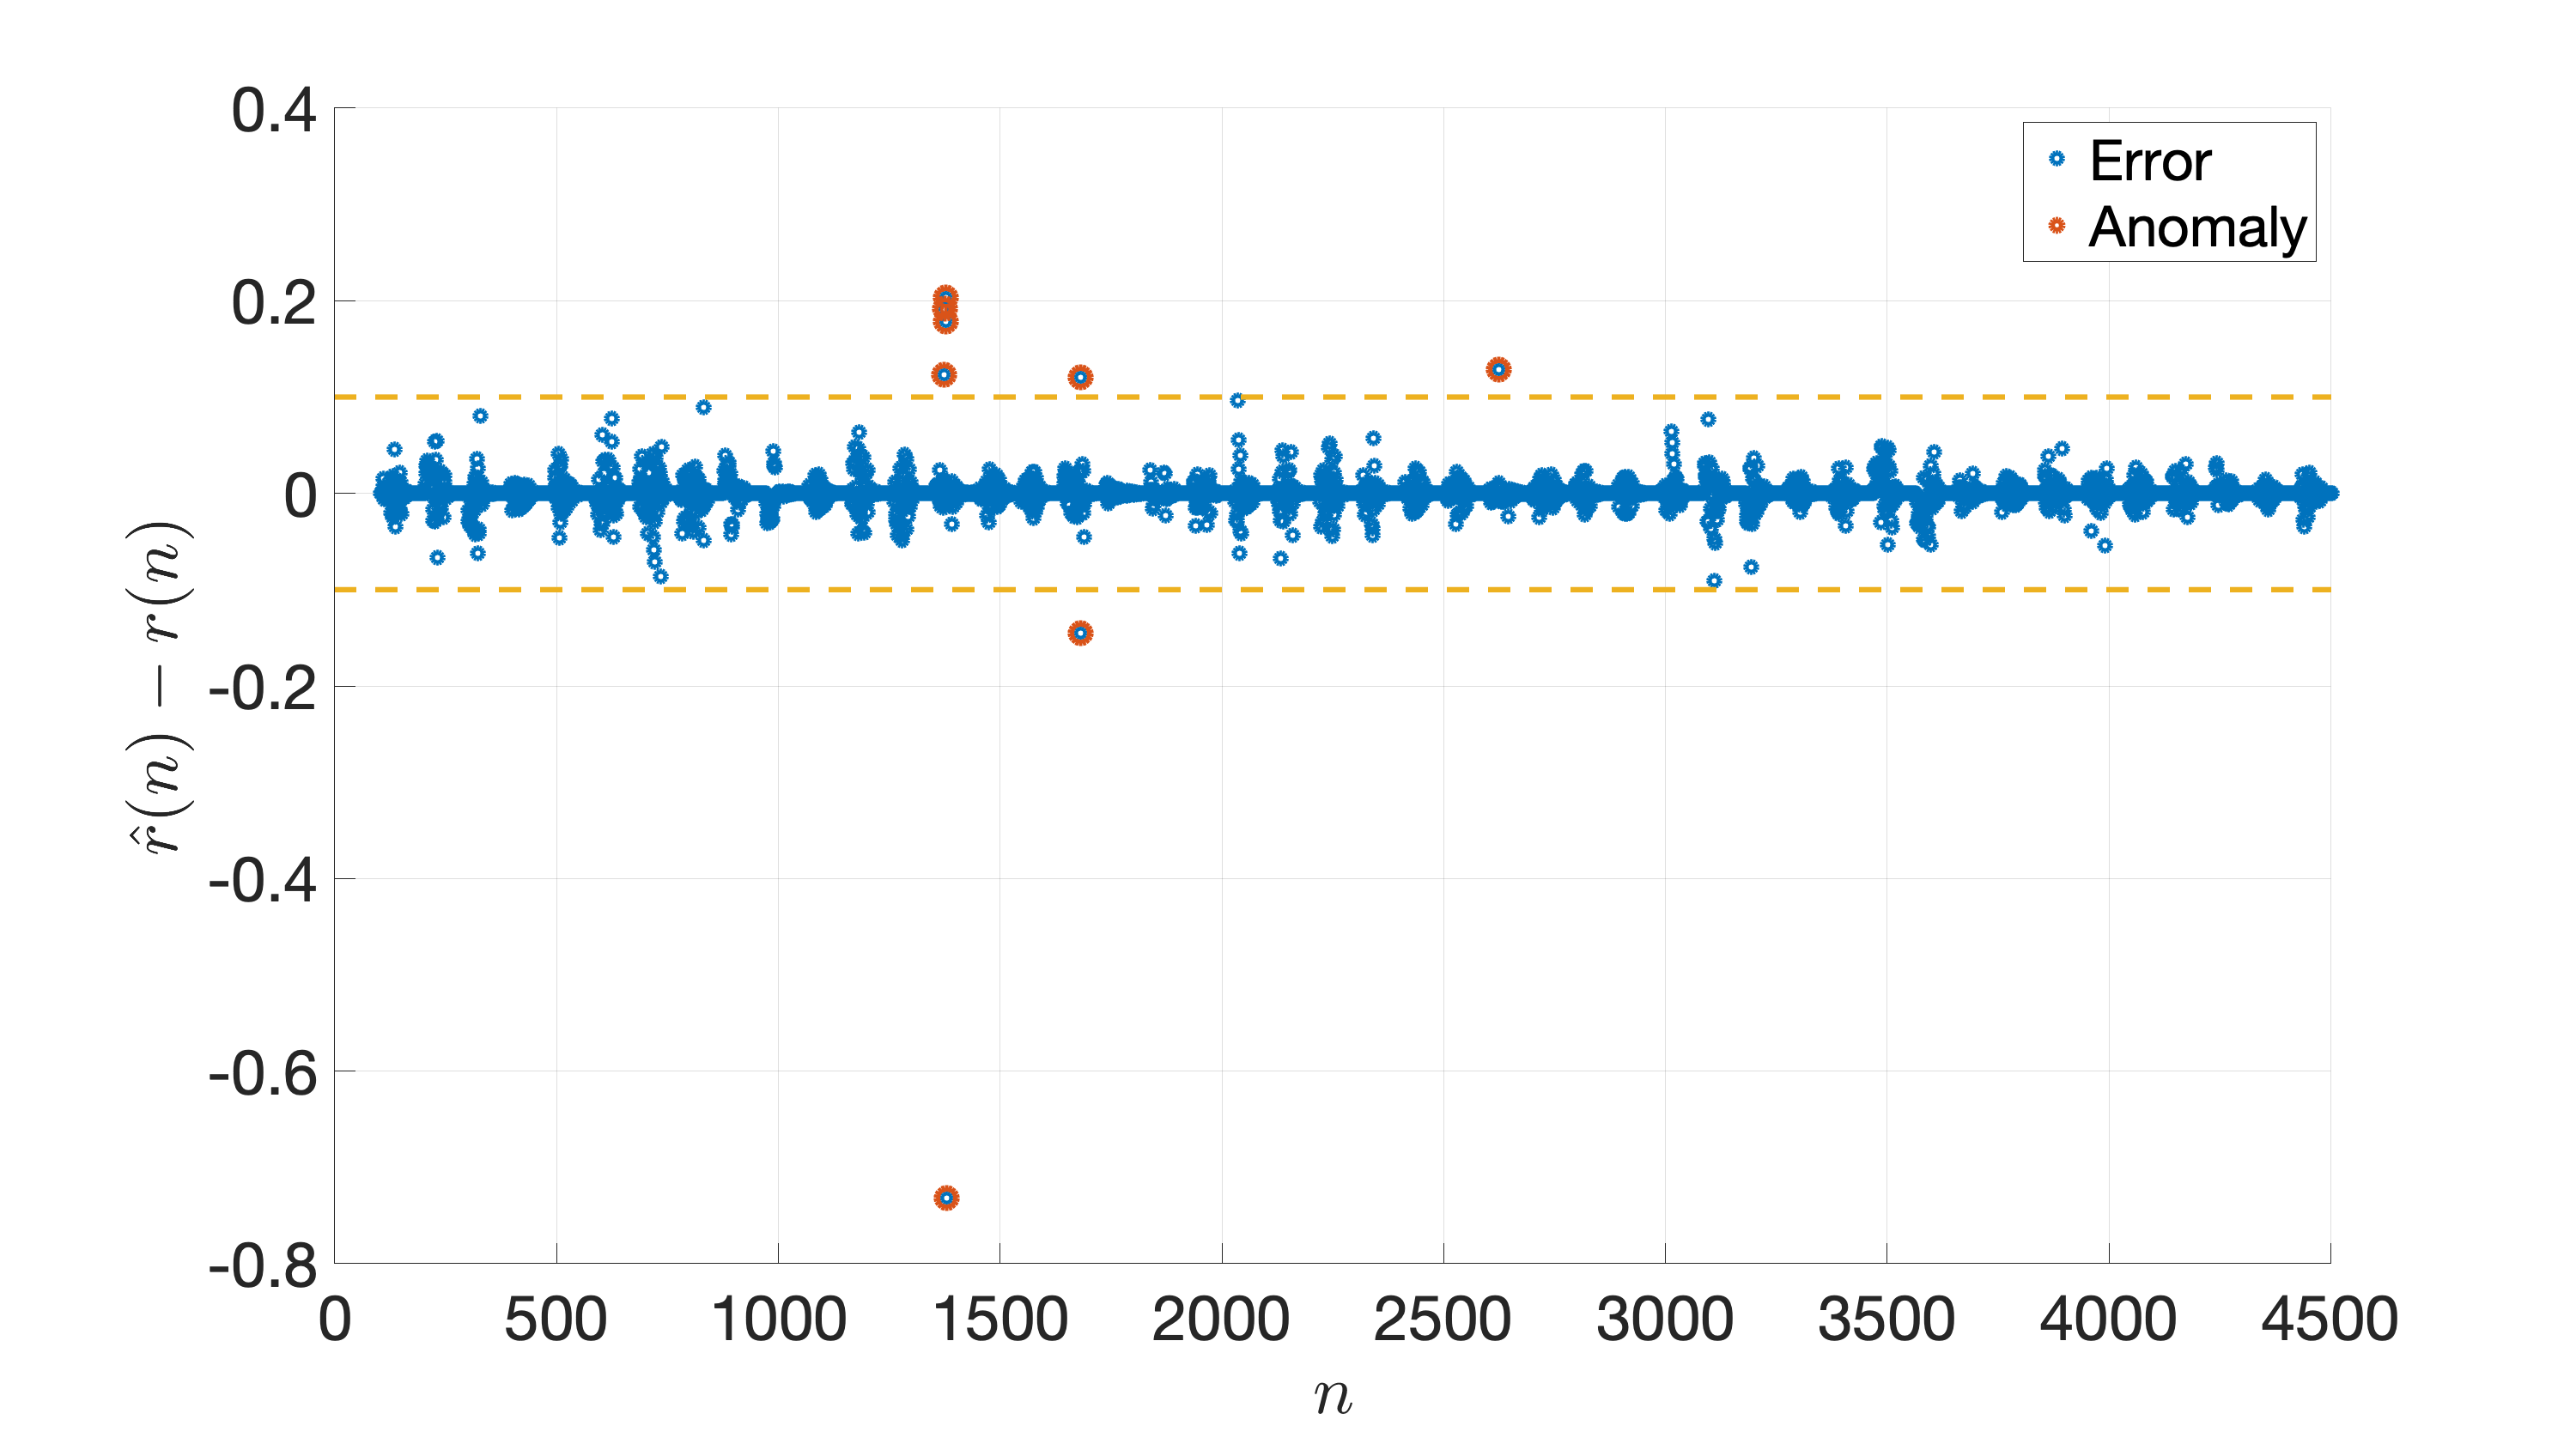
\includegraphics[width= 0.8\textwidth]{figures/R2c_error_an_after.png}
	\caption{Residue prediction error and anomaly identification after the test data is not dependent on the first anomalies found.}
	\label{fig:R2c_error_an_after}
\end{figure}

The second method, is simpler and computationally more efficient, but just because of the simplicity of the long-term prediction. This method follows three steps as well. First, the same first step as in the previous method is followed, identifying the intervals of time which are, without doubt, contaminated with an anomaly. In addition, the test data set in the intervals of time identified is substituted by the long-term prevision based on the previous day. Second, the long and short term predictions are computed based on the modified dataset. Third, the residue prediction error is plotted and the test for anomalies is run. Note that, given that the error is relative to the modified dataset, the regions identified in step one, are no longer identified. Fig. \ref{fig:R2c_error_an_after_m2} shows the residue estimation error relative to the modified set. It is noted that there are no regions with anomalies, which is consistent with the result obtained with the first method. It confirms, once again, the suspicion that the second anomalies being flagged in Section \ref{sec:r2b} were artificially flagged because of the dependence on the previous day, which was anomalous. It is also possible to see in this figure that the residue estimation error is null in the regions identified in step one, because is it the error relative to the modified set, which as forced to agree with the long term-prediction of the previous day.

\begin{figure}[htbp]
	\centering
	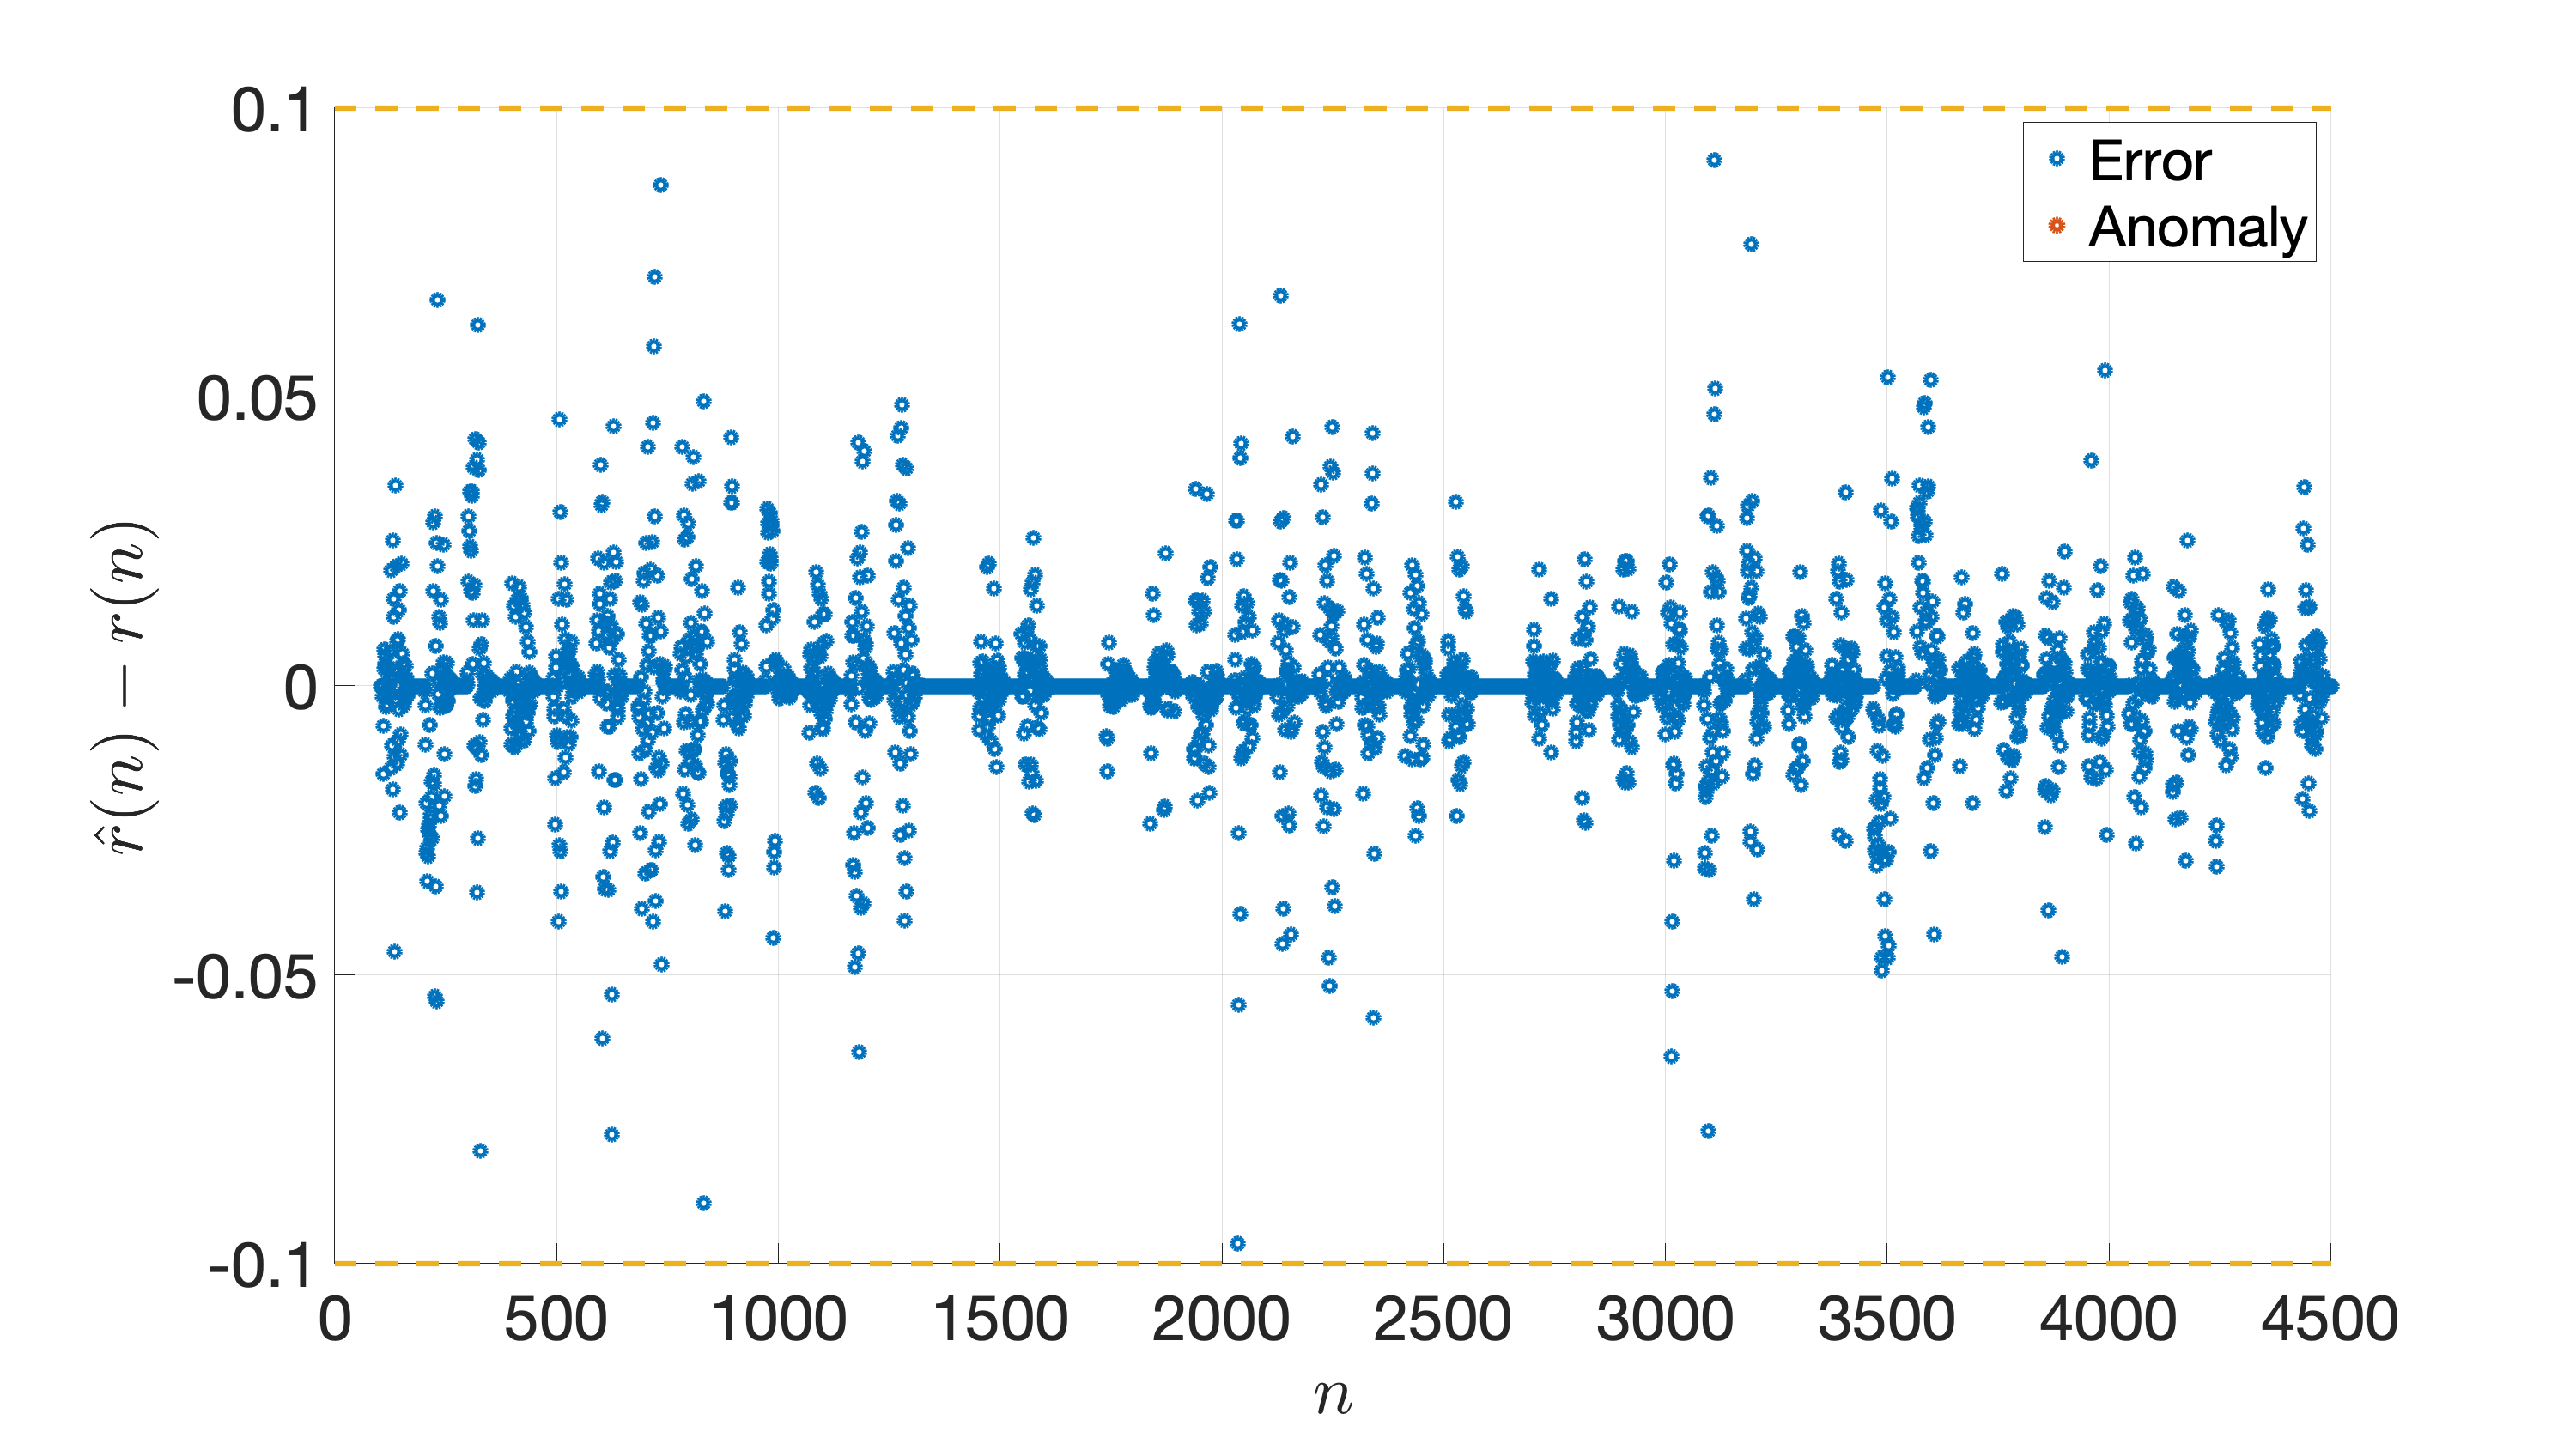
\includegraphics[width= 0.8\textwidth]{figures/R2c_error_an_after_m2.png}
	\caption{Residue prediction error and anomaly identification after the test data is not dependent on the first anomalies found, using the second method.}
	\label{fig:R2c_error_an_after_m2}
\end{figure}

\end{document}
